% !TEX program = xelatex
\documentclass[a4paper, 12pt]{article}

\setlength{\hoffset}{-1.6cm} 
\setlength{\voffset}{-1.6cm}
\setlength{\textheight}{24.0cm} 
\setlength{\textwidth}{17cm}

\usepackage{float} %použití [H] u figur, umístění na přesné místo
\usepackage{amssymb}
\usepackage[intlimits]{amsmath}
\usepackage{xltxtra,polyglossia}
\usepackage{tikz} % Export grafů z RStudia
\usepackage{placeins} % Umožňuje používat \FloatBarrier
\usepackage[super,square]{natbib} % Citace s horním indexem a v hranatých závorkách
\usepackage[nottoc]{tocbibind} % Aby se texal "Seznam použité literatury" místo "Reference"
\usepackage{color,graphicx,graphics}
\usepackage{booktabs,paralist,url}
\usepackage{pdfpages}
\usepackage{fancyhdr}
%\usepackage{siunitx} %$$\SI{666\pm 5 e3}{cm^{-1}}$$

\setmainlanguage{czech}
\renewcommand{\d}[1]{\ensuremath{\operatorname{d}\!{#1}}} %pro psaní \d jako derivace
\newcommand{\U}[1]{{\ \rm #1}} % sazba jednotek
\newcommand{\E}[1]{\cdot 10^{#1}} % sazba exponentu (10^exponent)
\newcommand{\EU}[2]{\E{#1}\U{#2}} % sazba exponentu a jednotek jednotek


\usepackage{newfloat} %pro zadefinování graph
\DeclareFloatingEnvironment{graph} %zadefinuje graph
\addto\captionsczech{ %vytvoří 2 typy figur
  \renewcommand{\graphname}{Graf} %\begin{graph}
  \renewcommand{\figurename}{Obrázek}%\begin{figure}
}
%\bibliography{literatura}
%\input{dependencies/slovnik} % explicitní slovník slov, která se mají zalamovat na konci řádku ( nejnovější verze vždy na https://gitlab.com/skolar/slovnik.git )

%\usepackage{fkssugar}
%\usepackage{longtable}
%\usepackage{python}

%pro pdfTEX
%\usepackage[utf8]{inputenc}
%\usepackage[T1]{fontenc}
%\usepackage{lmodern}
%\usepackage[czech]{babel}

%tikz input
\usepackage{pgfplots}

\newlength\figureheight
\newlength\figurewidth

% \newcommand{\AUTOR}{}

% \usepackage{fancyhdr}
% \pagestyle{fancy}
% \lhead{}
% \rhead{\AUTOR}

\begin{document}
\section{Moučný červ (Tribolium)}
Aby bylo možné počítat populace moučných červů, je nutné znát jejich životní cyklus. Z fundamentáního pozorování jejich vývoje lze tento cyklus odhadnout. Prvotní fází je vajíčko ($L$), z nějž se po 2 týdnech vylíhne larva ($P$). Po dalších dvou týdnech se z larvy stává dospělý červ ($A$). Vývoj jednotlivých fází lze popsat vztahy\\
\begin{equation}
    \begin{split}
\text{Larva: }& L_{n+1}=b A_n \\
\text{Kukla: }& P_{n+1}=L_n(1-\mu_l) \\
\text{Brouk: }& A_{n+1}=P_n(1-\mu_p)+A_n(1-\mu_a), \\
    \end{split}
\end{equation}
kde $\mu_l$ je úmrtnost larev, $\mu_p$ úmrtnost kukel a $\mu_a$ úmrtnost brouků. Spodní indexy jsou pak ordinálním číslováním populace.


Pokud zahrneme kanibalismus, který se u těchto druhů často vyskytuje, dostaneme: \\
\begin{equation}
\label{eq:vyvoj}
\begin{split}
\text{požírání larev: }&L_{n+1}=b A_n e^{-c_{la}A_n-c_{ll} L_n} \\
\text{požírání kukel: }&P_{n+1}=L_n(1-\mu_l) \\
\text{požírání brouků: }& A_{n+1}=P_n(1-\mu_p)e^{-c_{pa} A_n}+A_n(1-\mu_a), \\
\end{split}
\end{equation}
kde koeficienty byly zjištěny experimentálně jako
\begin{equation}
\begin{split}
c_{la}& = 0.009 \text{ (A požírá L)}\\
c_{ll}& = 0.012 \text{ (L požírá L)}\\
c_{pa}& = 0.004 \text{ (A požírá P)}\\
\mu_l& = 0.267 \\
\mu_p& = 0\\
\mu_a& = 0.0036 \text{ (základní úmrtnost)} \\
b& =7.48 \text{ počet nových larev na 1 dospělého brouka za jednotku času, což je 14 dní)}\\
\end{split}
\end{equation}
Všechny tyto parametry jsou tzv. řídící parametry systému.

\subsection{Bifurkační diagram}
Systém popsaný rovnicemi \ref{eq:vyvoj} tvoří pro některý interval řídících parametrů chaotický systém, tzn. že malé změny v počátečních podmínkách způsobí, že po několika desítkách až stovkách cyklech může být rozdíl v počtu jedinců velký. Pro vizualizaci limitních stavů systému pro různé řídící parametry se využívá bifurkační diagram. Bifurkační diagram generujeme dostatečným počtem iterací systému (tím se dostaneme do limitního stavu) a následně uložením několika posledních hodnot pro danou hodnotu řídícího parametru (řádově desítky hodnot). Na bifurkačním diagramu pak vidíme zdvojování period (pro jednu hodnotu parametru dostáváme více limitních hodnot) a pokud systém přejde do chaotického režimu, dostáváme pro jednu hodnotu řídícího parametru velké množství limitních hodnot. V našem případě byla zvolena osa $x$ pro úmrtnost brouků $\mu_a$ a osa $y$ pro počet jedinců po 200-230 cyklech.
% \setlength\figureheight{2in}
% \setlength\figurewidth{3in}
% \InputIfFileExists{grafy/bifurcation.tikz}{}{\textbf{!! Missing graphics !!}}
\begin{graph}[H]
	\centering
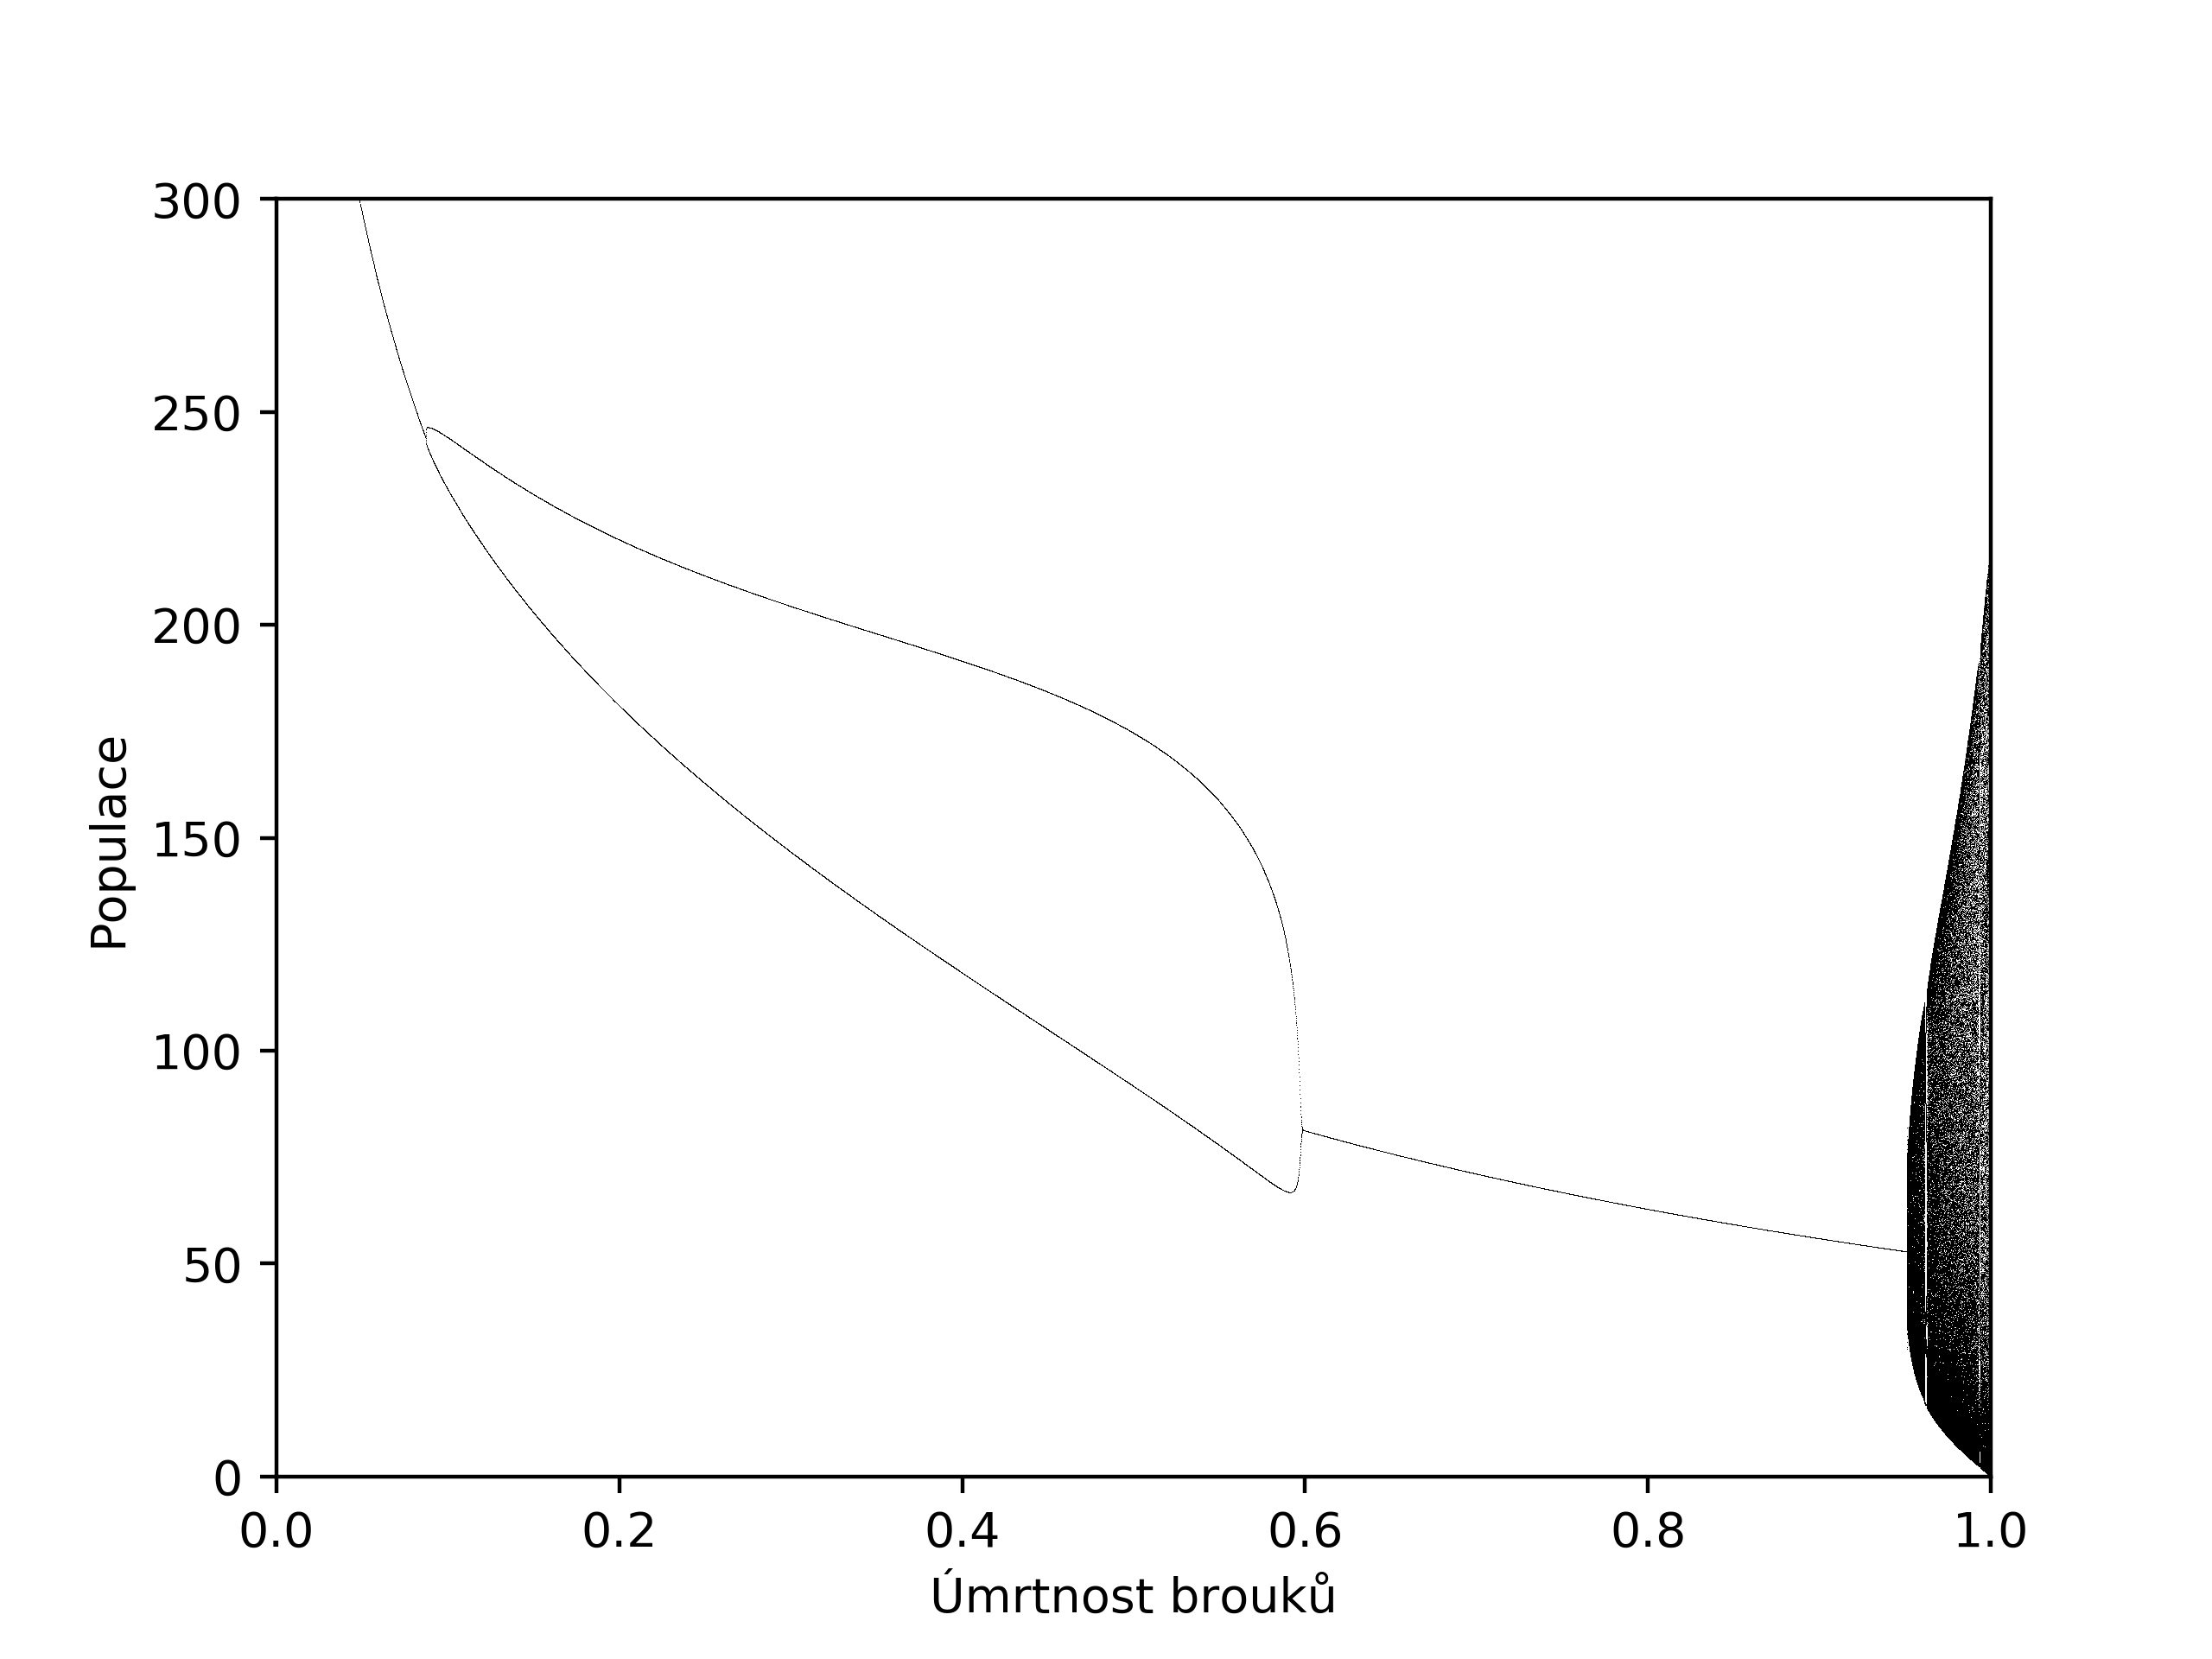
\includegraphics[width=\textwidth]{grafy/bifurcation.png}
\vspace{-10pt}
\caption{Bifurkační diagram}
\label{fig:bifurcation}
\end{graph}

Z grafu \ref{fig:bifurcation} je patrné, že k první bifurkaci dochází při $\mu_a=0.1$, kde se perioda $1$ mění na periodu $2$. Druhá bifurkace je v bodě $\mu_a=0.6$, perioda $2$ se mění na $1$. ke třetí bifurkaci dochází při $\mu_a=0.954$, kde se systém začíná chovat chaoticky.

\begin{graph}[H]
	\centering
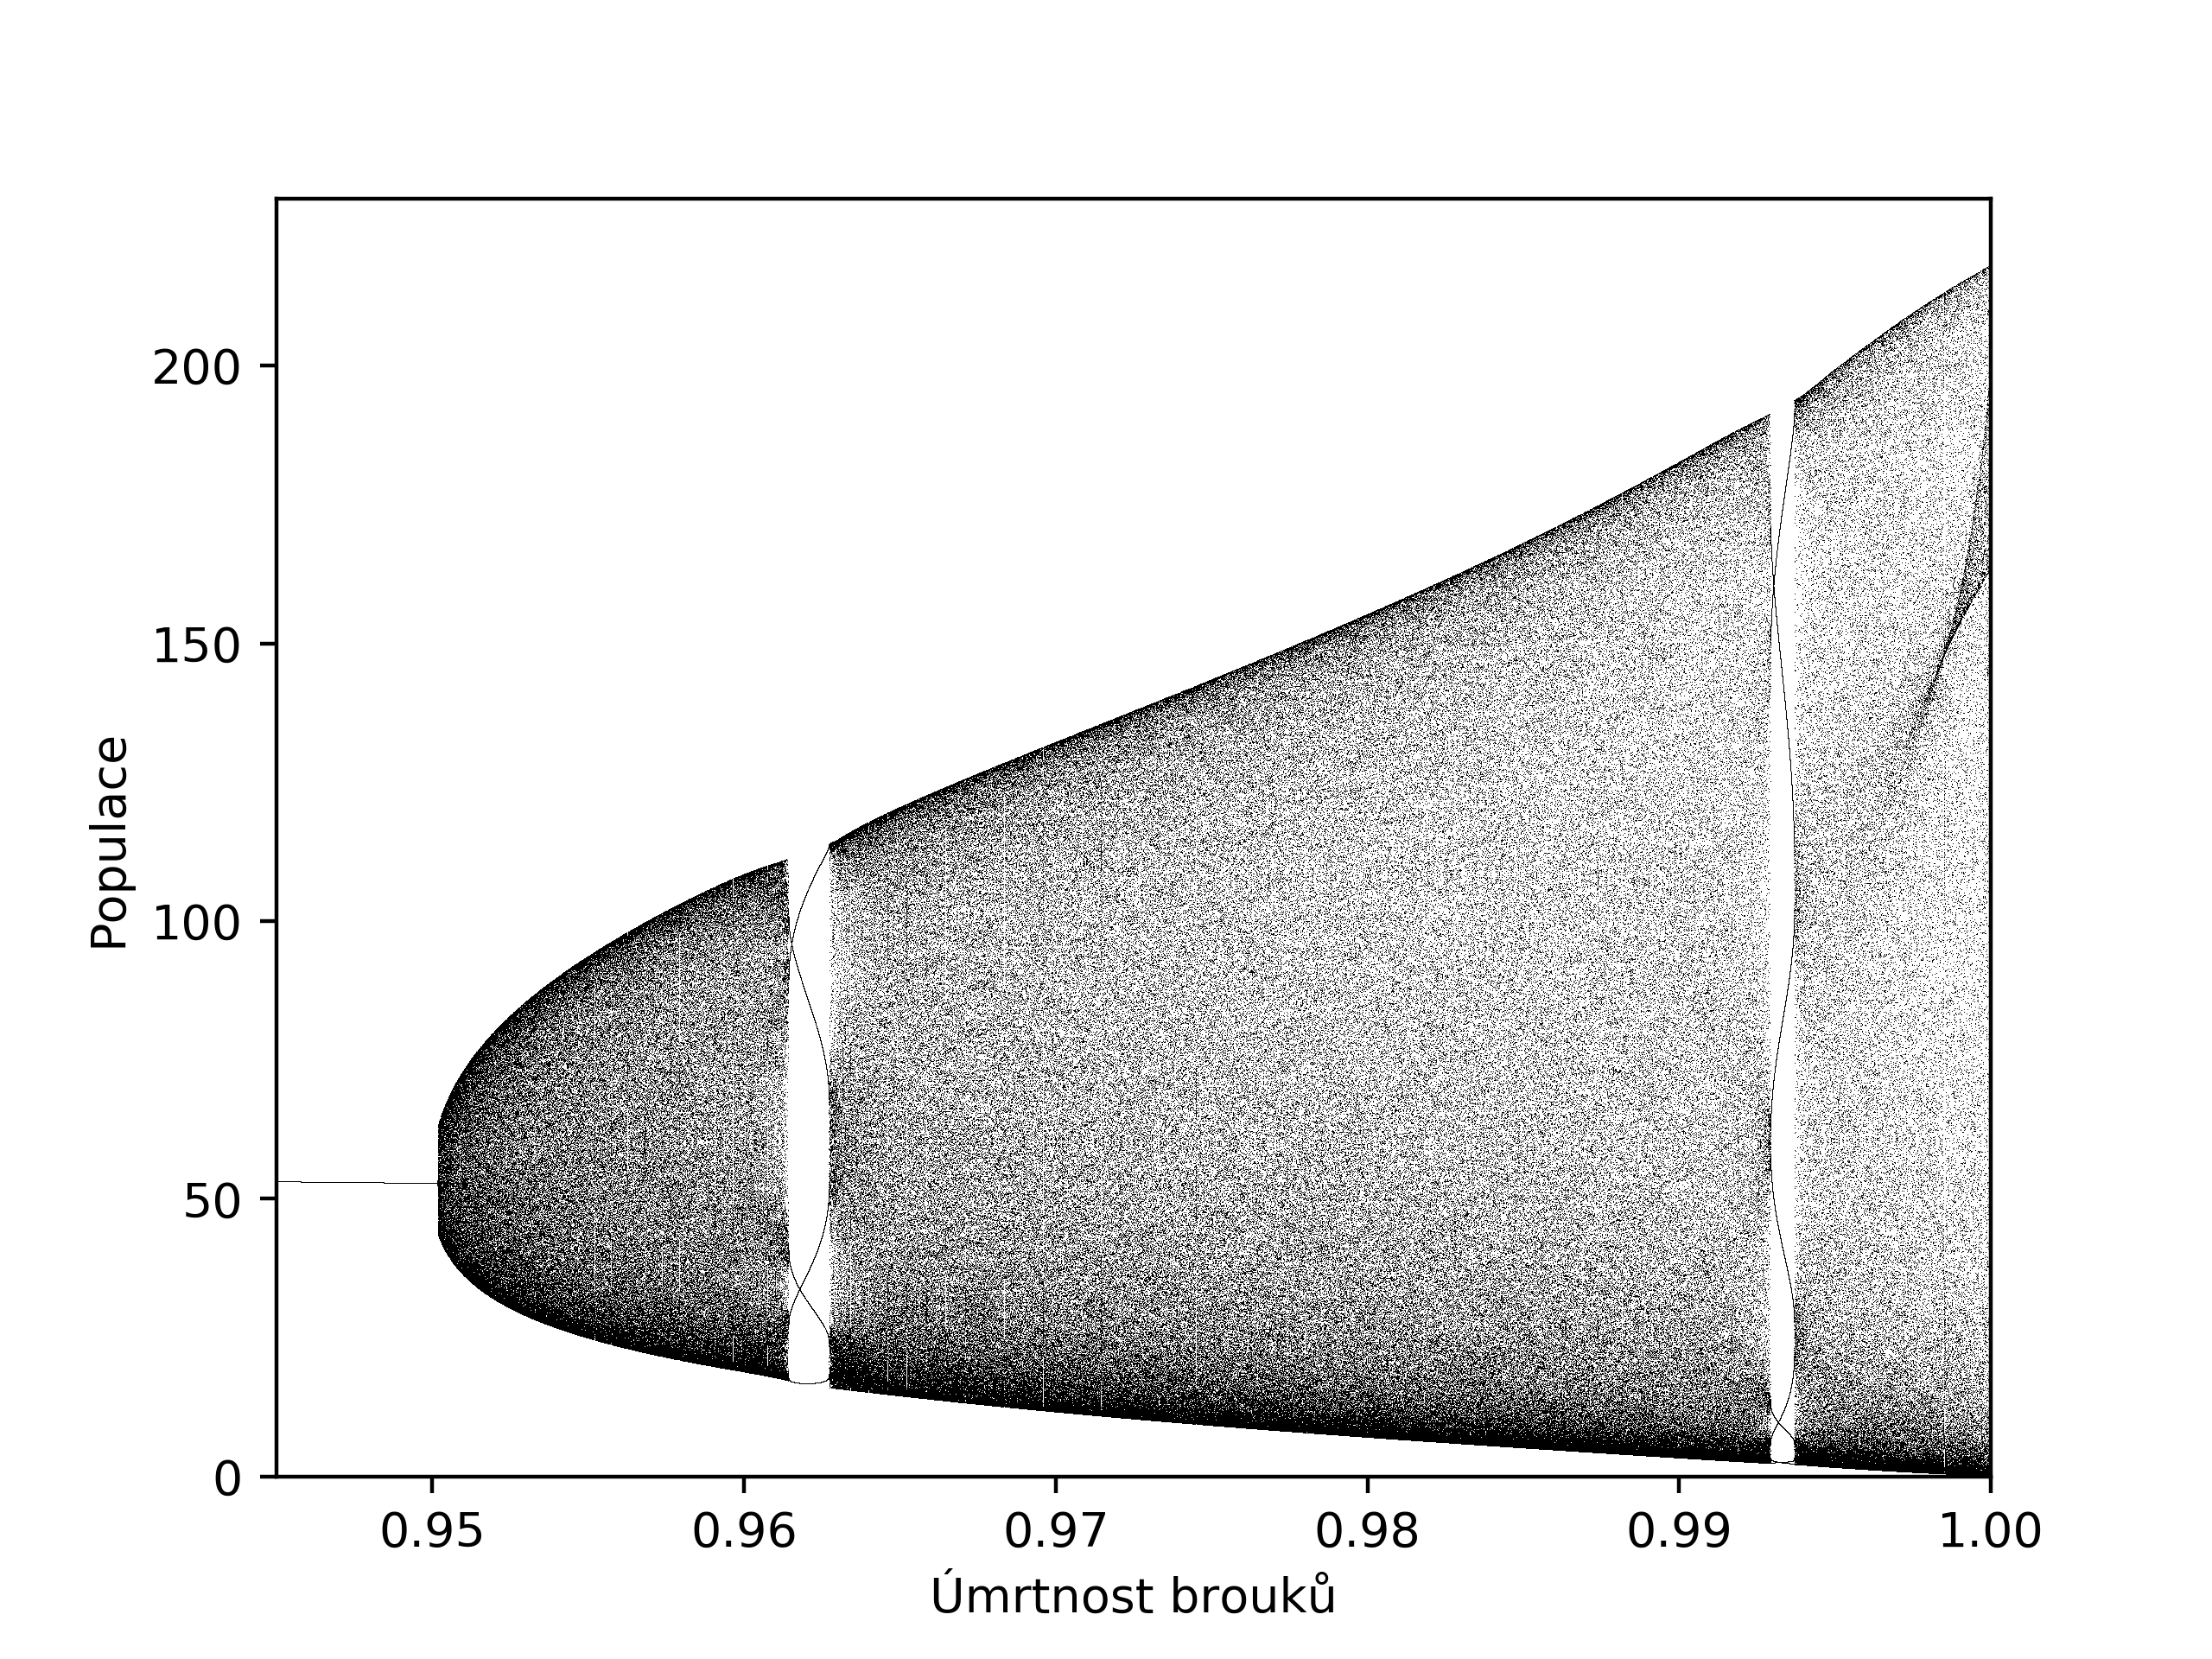
\includegraphics[width=\textwidth]{grafy/bifurcation_zoom2.png}
\vspace{-10pt}
\caption{Bifurkační diagram - přiblížení na chaotický režim}
\label{fig:bifurcation_zoom}
\end{graph}

\subsection{Nalezení největšího Ljapuova exponentu}
Pro nalezení největšího Ljapuova exponentu pro $\mu_a\in[0,1]$ jsme nejdříve systém s počátečními podmínkami $L_0=100, P_0=100, A_0=100$ iterovali 400 generací aby jsme se při určování Ljapunova exponentu nacházeli na atraktoru. V konfiguračním prostoru jsme pak vytvořili druhou orbitu $\vec{x_b}$ přičtením vektoru $\vec{d_0}=\left(0,0,10^{-8}\right)$ ke stavovému vektoru $\vec{x_a}$ obdrženému po 400 iteracích od počátečních podmínek. Obě orbity jsme následně iterovali 3000 generací s tím, že po každé iteraci jsme uložili hodnotu $d=\frac{|\vec{x_b}-\vec{x_a}|}{|d_0|}$ a korigovali druhou orbitu vzorcem $\vec{x_{bkor}}=\vec{x_a}+\frac{1}{d}\left(\vec{x_b}-\vec{x_a}\right)$. Korigováním druhé orbity jsme zajistili, že vektor $\vec{x_{bkor}}$ je vždy ve vzdálenosti $|\vec{d_0}|$ od vektoru $\vec{x_a}$, ale ve směru $\vec{x_b}-\vec{x_a}$. Z uložených hodnot $d$ jsme určili průměr všech $log(d)$, který je maximálním Ljapunovým exponentem. 

\begin{graph}[H]
	\centering
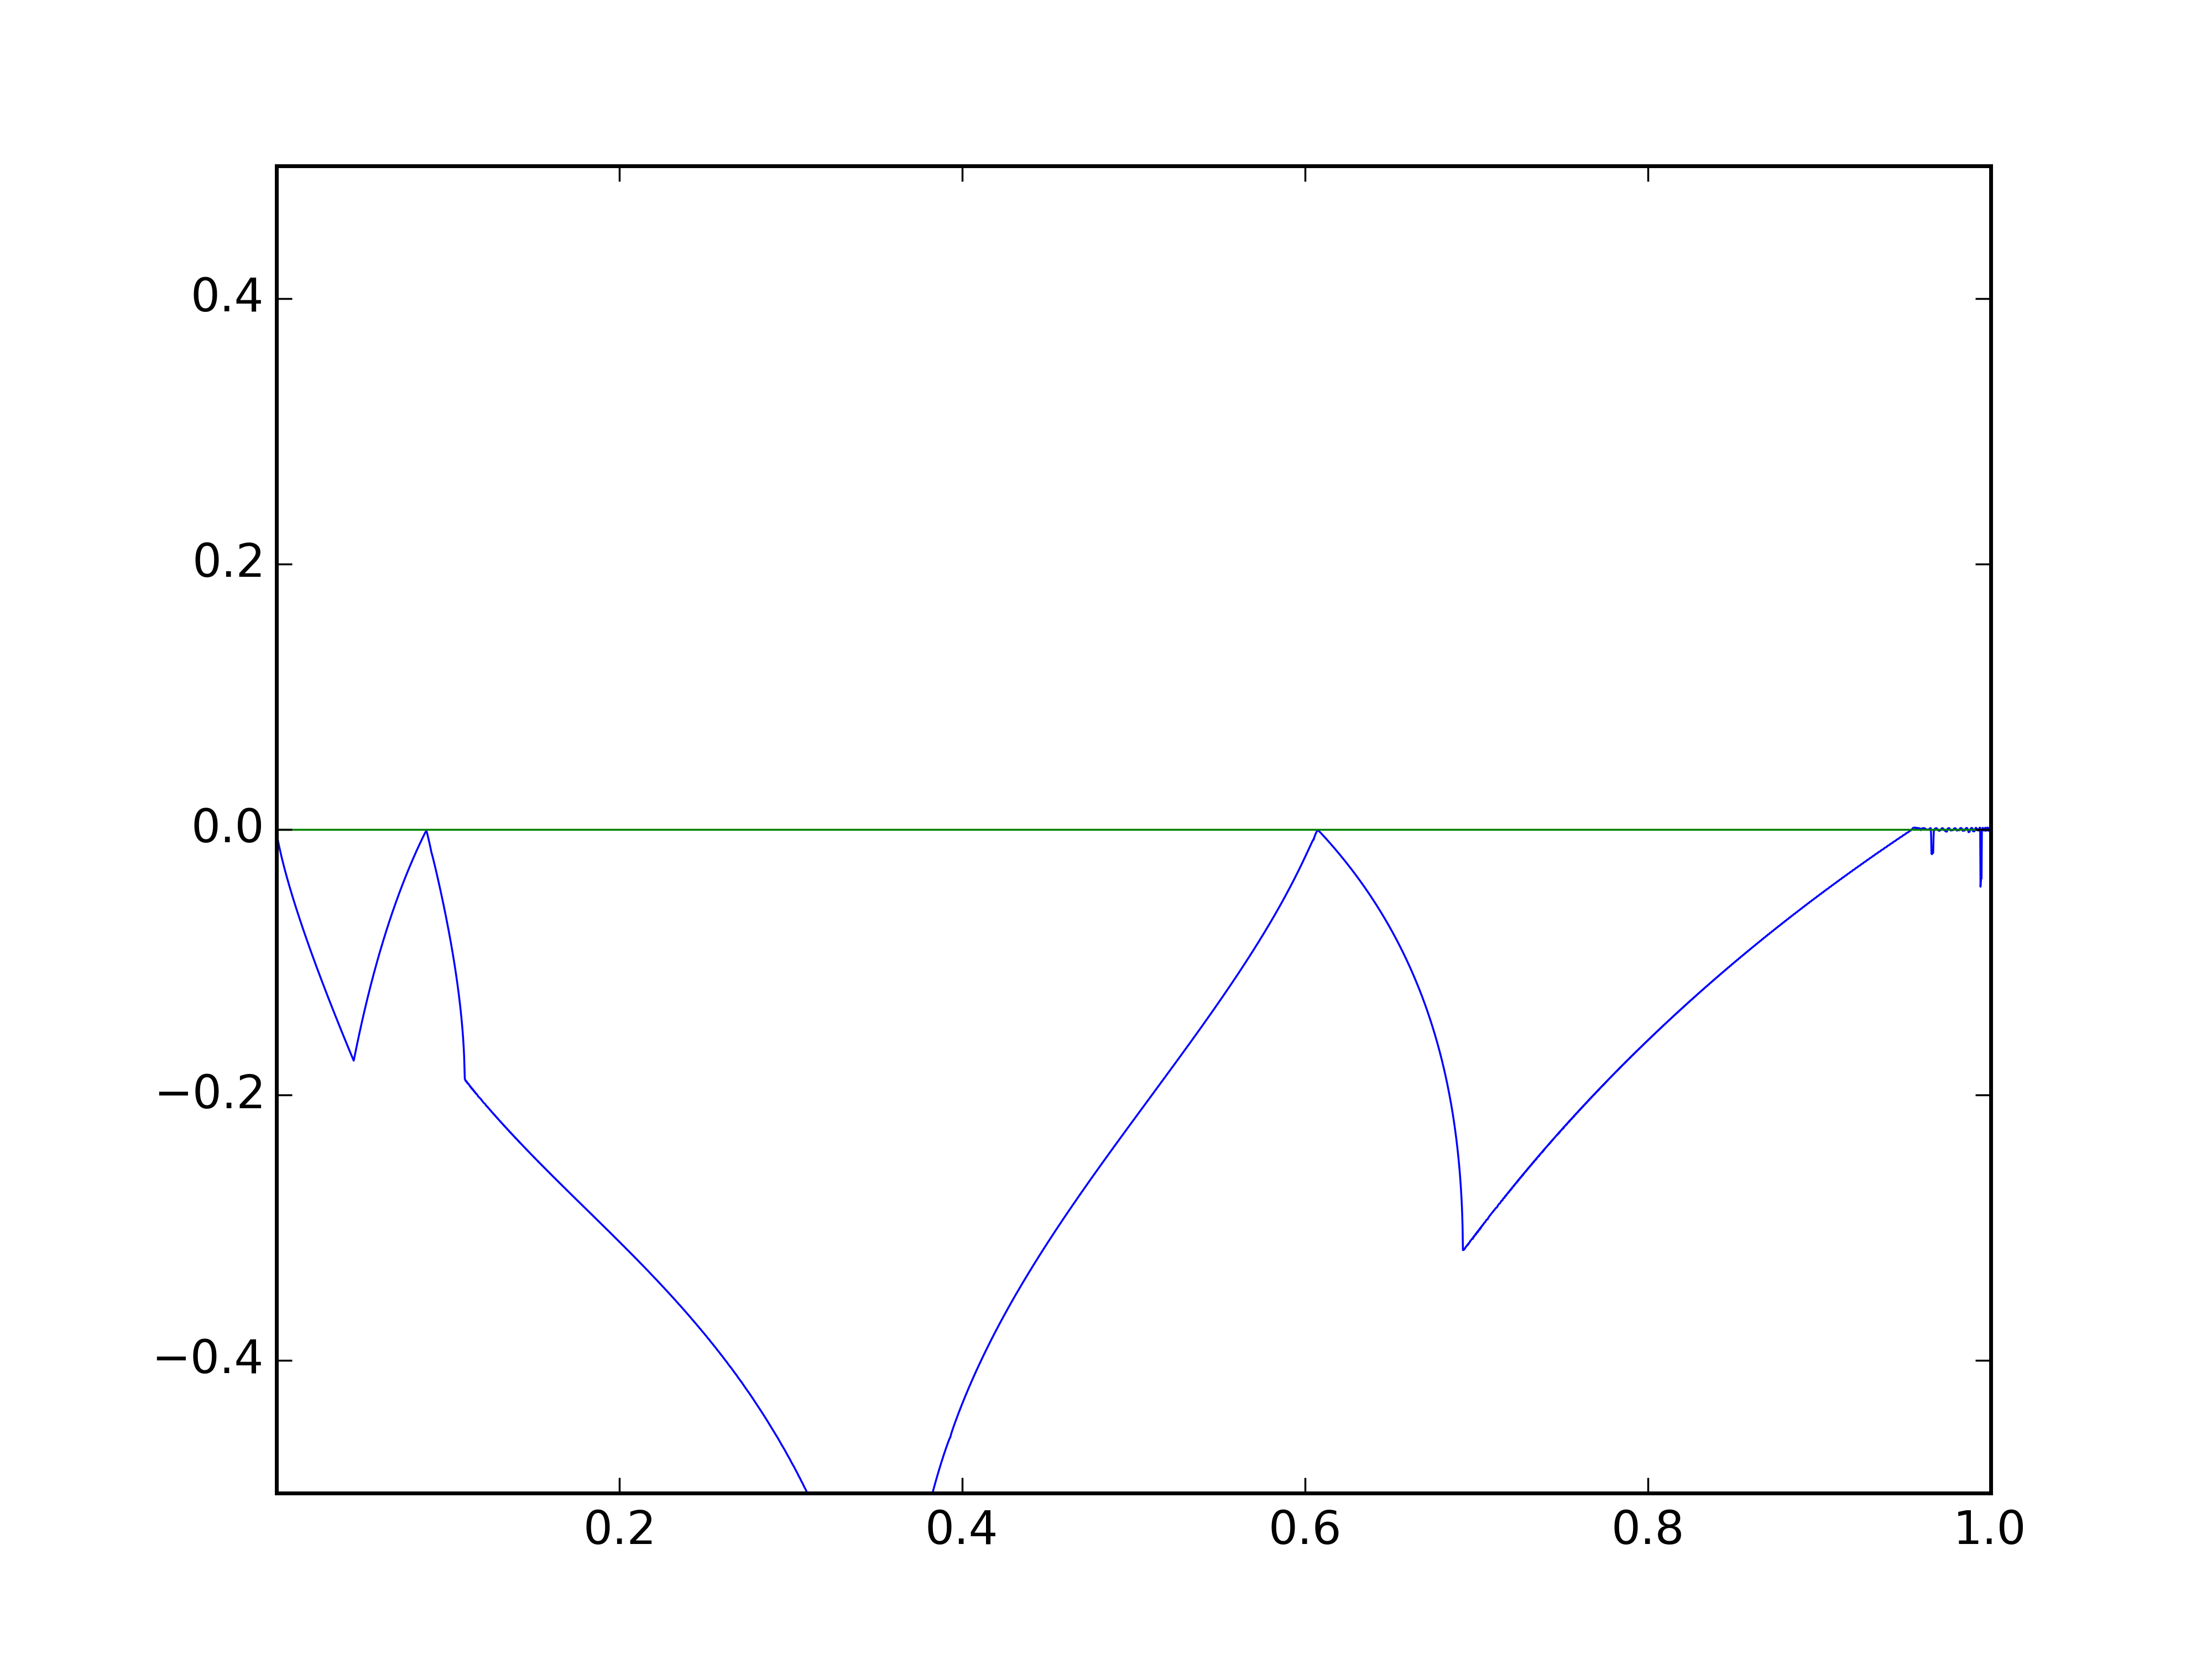
\includegraphics[width=\textwidth]{grafy/mua_f_wid.png}
\vspace{-10pt}
\caption{Maximální Ljapunovy exponenty pro parametr $\mu_a$}
\label{fig:lyapunov_mua}
\end{graph}

Z hodnot Ljapunových exponentů na grafu 3 vidíme, že v bodech kde dochází ke zdvojování periody orbity jde Ljapunův exponent do nuly, nad hodnotou $\mu_a=0.954$ systém přechází do chaotického režimu (Ljapunův exponent je zde kladný, což je vidět na grafu 4), vidíme ale intervaly řídícího parametru v oblasti $\mu_a > 0.954$, kde dochází k dalším bifurkacím (jak je vidět na bifurkačním diagramu) a exponent je záporný.

\begin{graph}[H]
	\centering
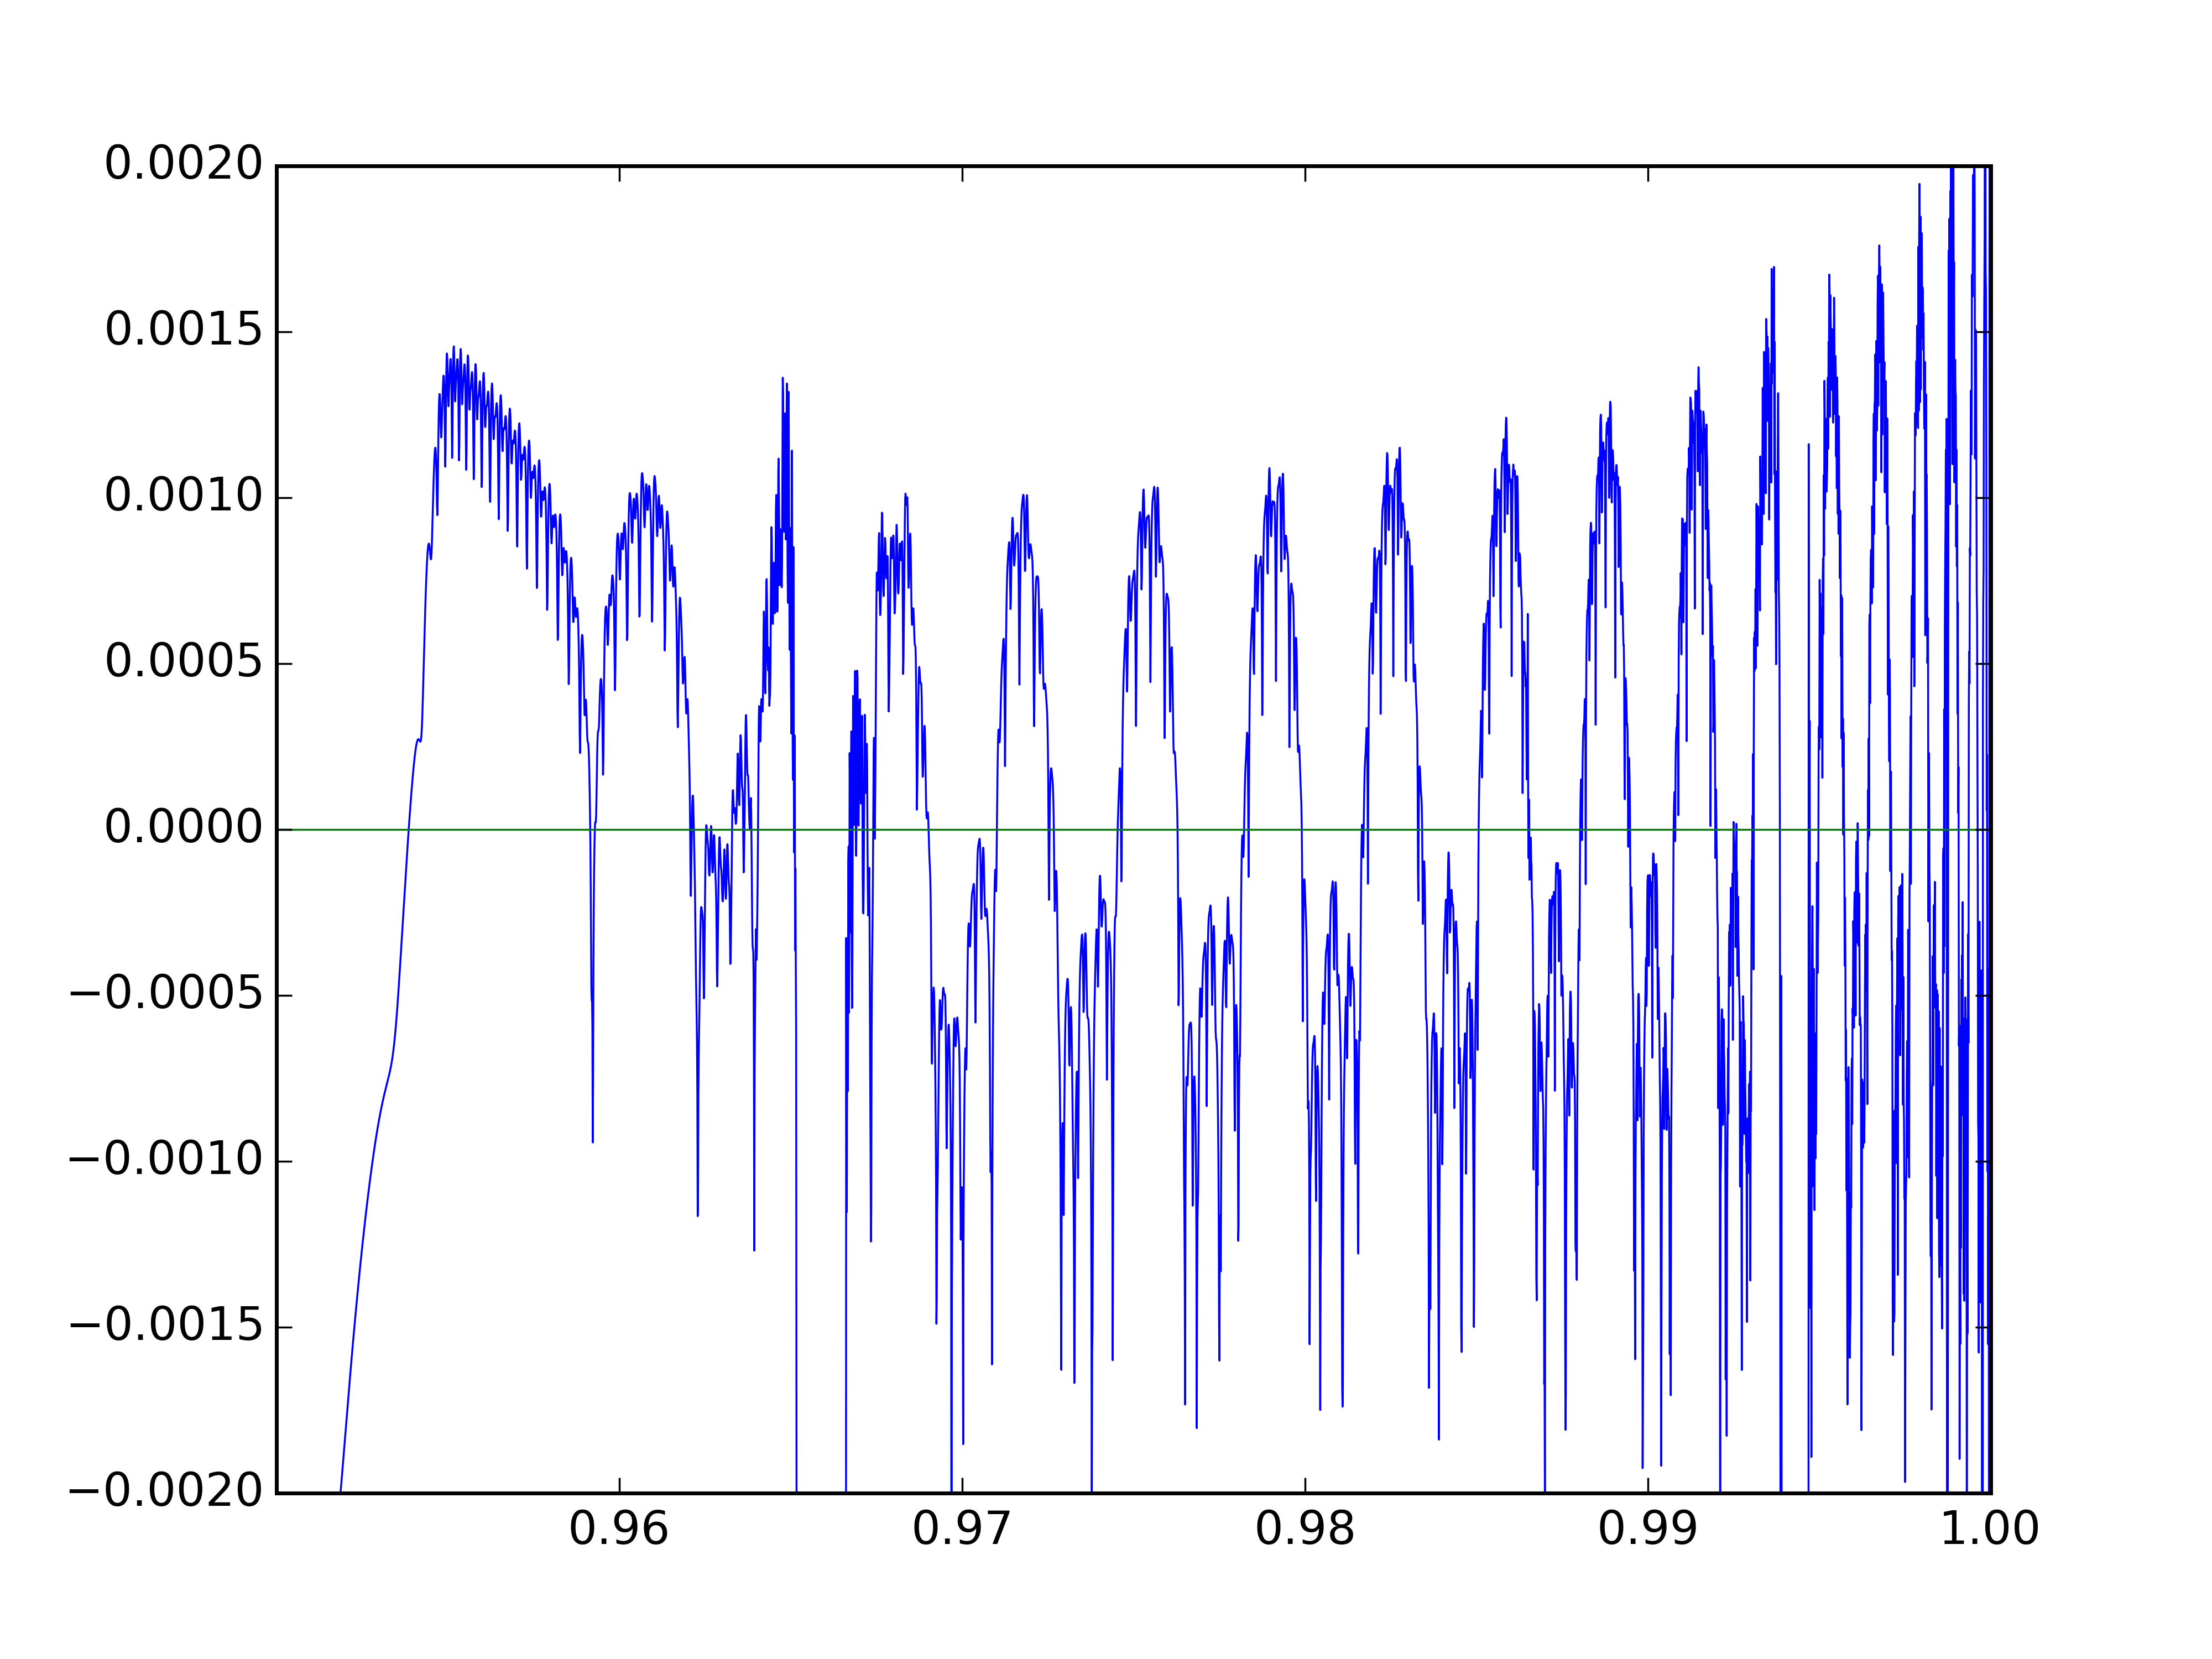
\includegraphics[width=\textwidth]{grafy/mua.png}
\vspace{-10pt}
\caption{Ljapunovy exponenty pro paremetr $\mu_a$, přiblížení na chaotický režim}
\label{fig:lyapunov_mua_zoom}
\end{graph}

---------------------------------------------------------------------\\
\today, Daniel Rod, Michal Grňo, Jan Střeleček

\end{document}